%!TEX root = ../main.tex

%
% Notes: 
%
%  exact implementation
%  comparison with rollback at batch N
%  relaxing the solvers
%  dealing with false positives
%
%  running on TPC-C/sanjay's.  equality is easier
%
% Need names for
%  * rollback
%  * exact solution
%  * fixing an individual/batch of queries
%
\section{Experiments}
\label{sec:experiments}


  \begin{figure*}[h]
  \centering
    \vspace*{-.2in}
    \begin{subfigure}[t]{.3\textwidth}
    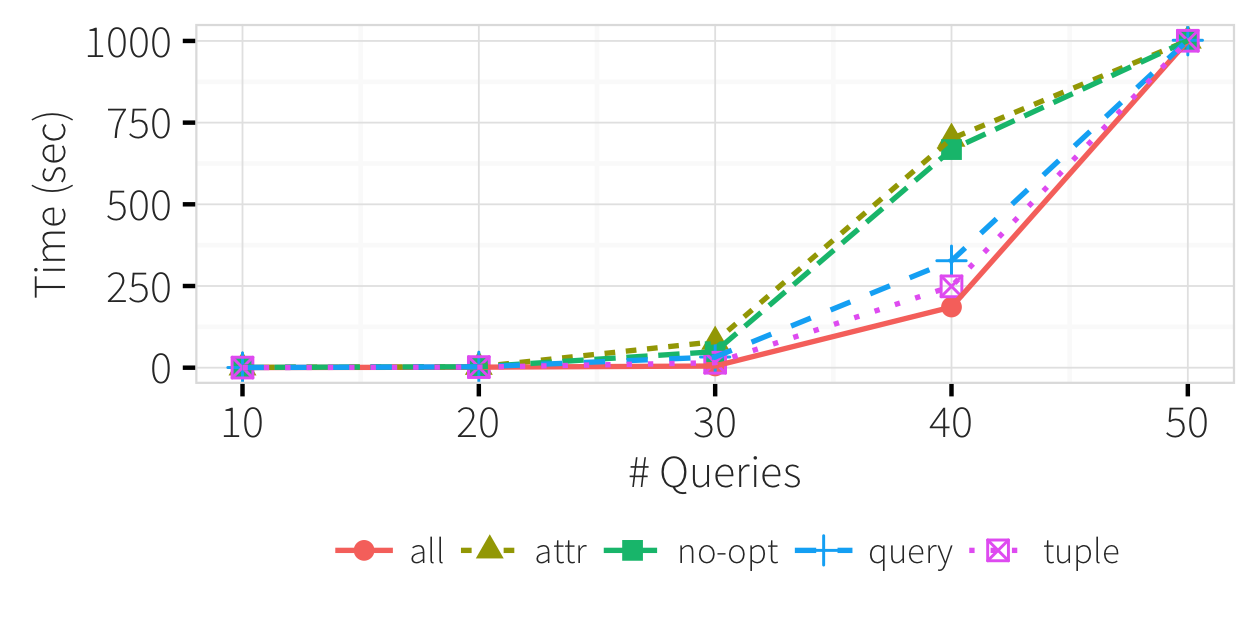
\includegraphics[width = .99\columnwidth]{figures/multi_time}
    \vspace*{-.25in}
    \caption{Performance for multiple corruptions.}
    \label{f:multi_time} 
    \end{subfigure}
    \begin{subfigure}[t]{.3\textwidth}
    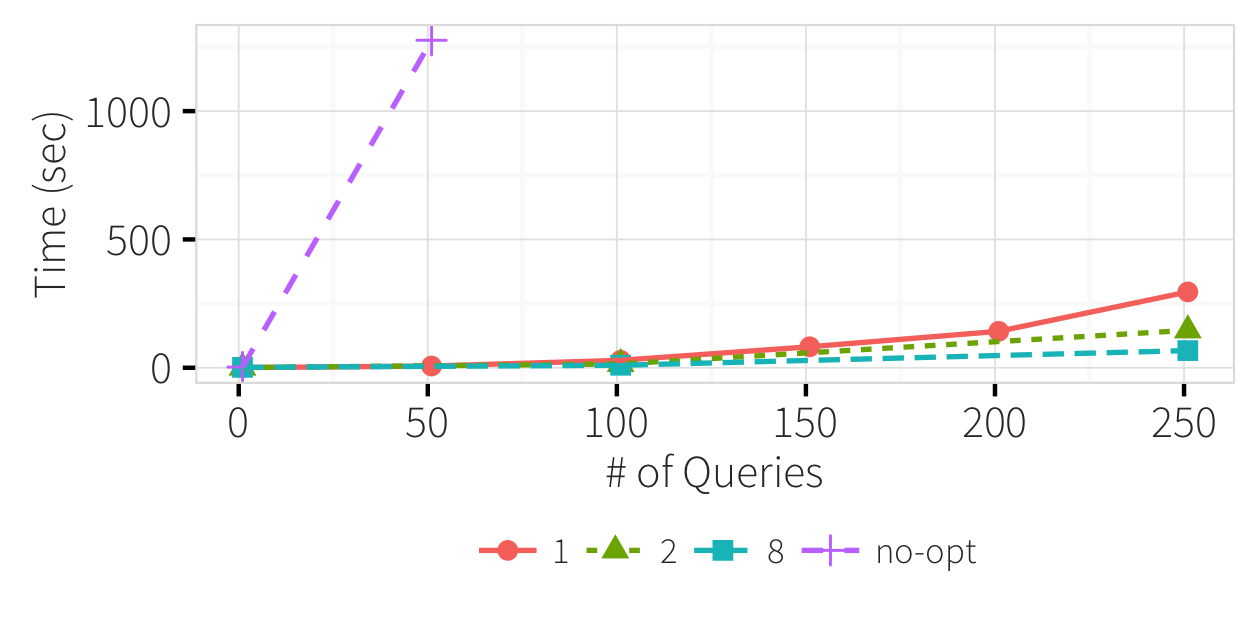
\includegraphics[width = .99\columnwidth]{figures/incrementalcompare_time}
    \vspace*{-.25in}
    \caption{Performance for single corruption.}
    \label{f:singlequeryinc_time} 
    \end{subfigure}
    \begin{subfigure}[t]{.3\textwidth}
    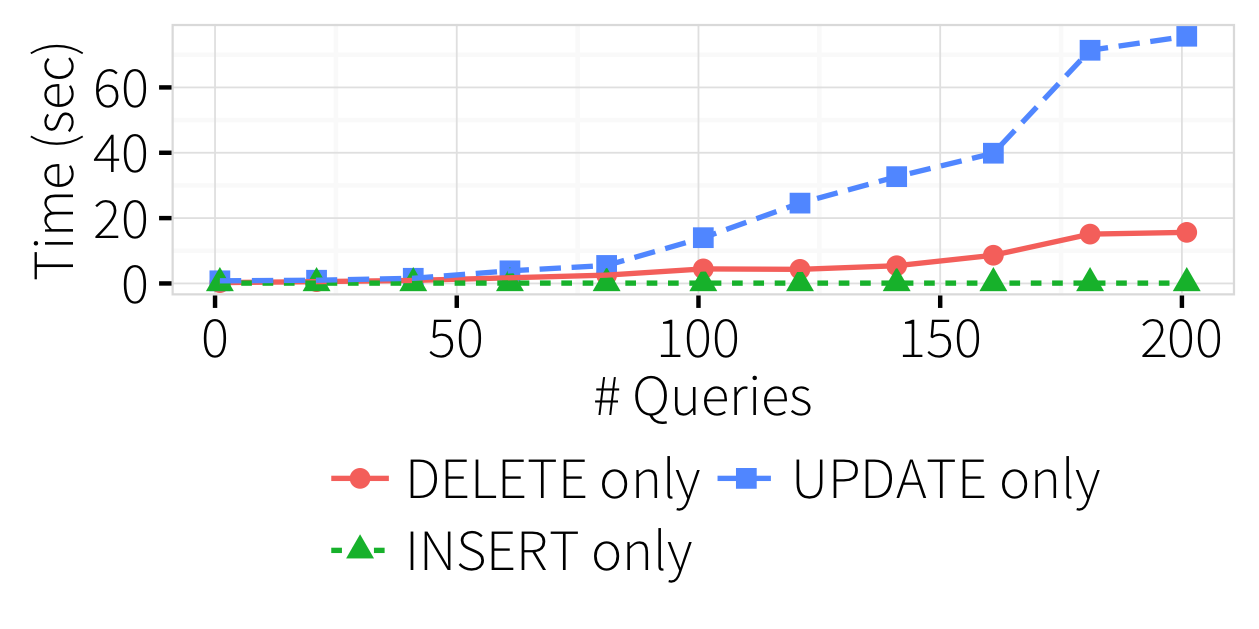
\includegraphics[width = .99\columnwidth]{figures/indelup_time}
    \vspace*{-.25in}
    \caption{Performance for different query types.}
    \label{f:indelup_time} 
    \end{subfigure}
    \\
    \begin{subfigure}[t]{.3\textwidth}
    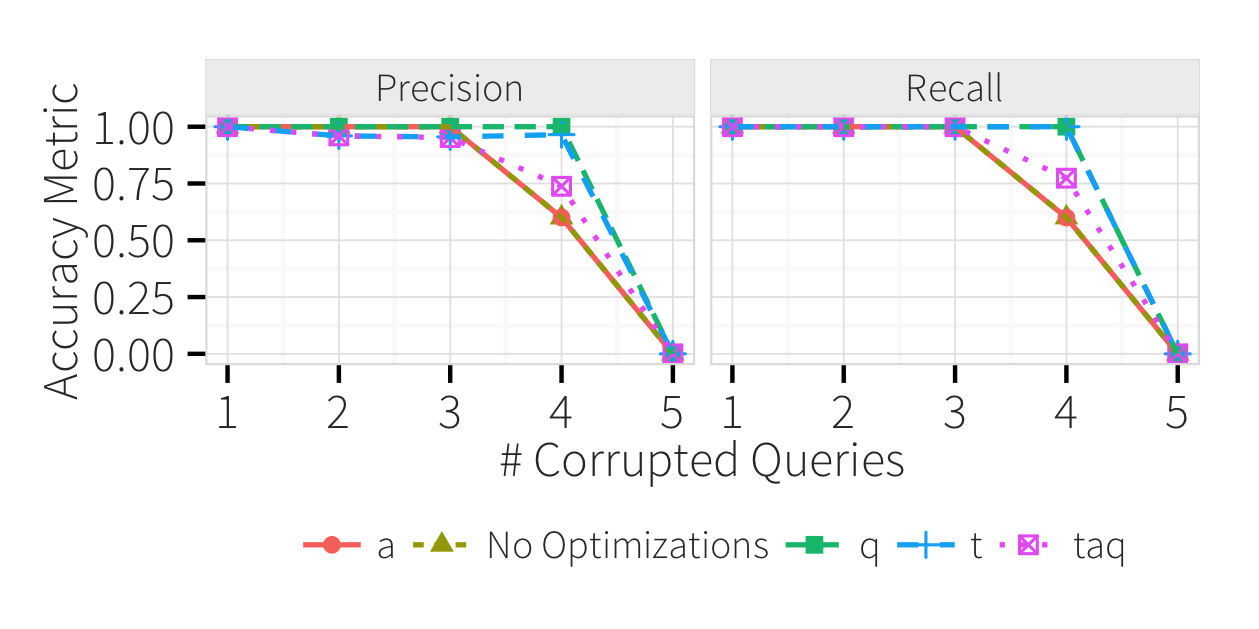
\includegraphics[width = .99\columnwidth]{figures/multi_pr}
    \vspace*{-.25in}
    \caption{Accuracy for multiple corruptions.}
    \label{f:multi_acc} 
    \end{subfigure}
    \begin{subfigure}[t]{.3\textwidth}
    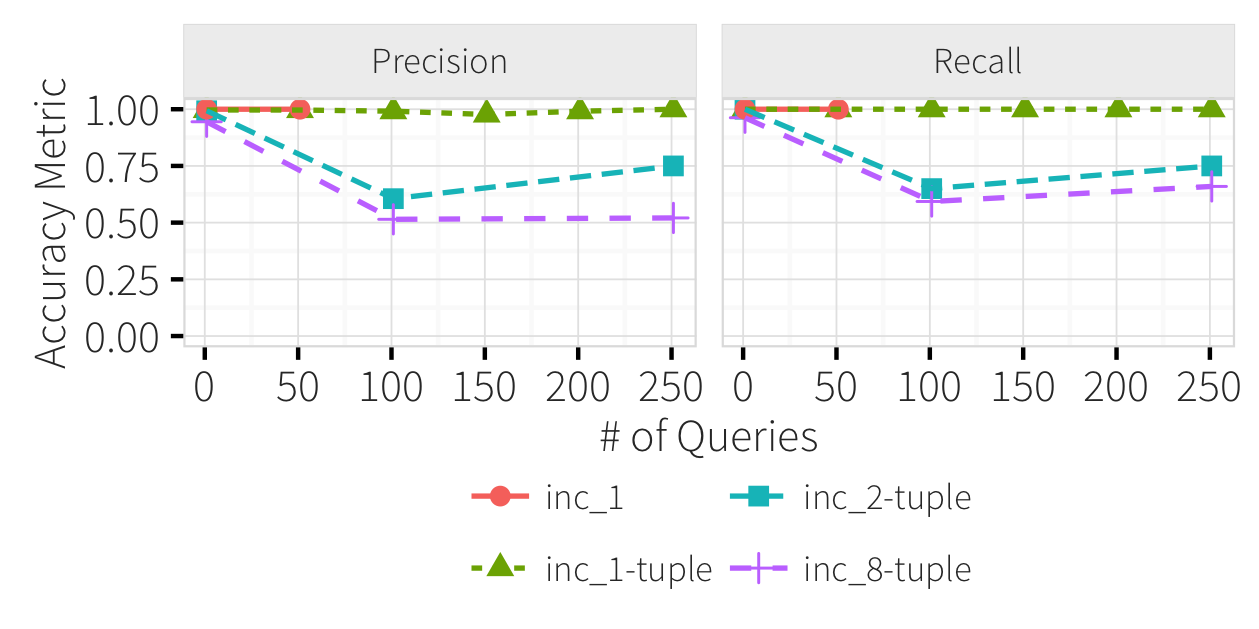
\includegraphics[width = .99\columnwidth]{figures/incrementalcompare_acc}
    \vspace*{-.25in}
    \caption{Accuracy for single corruption.}
    \label{f:singlequeryinc_acc} 
    \end{subfigure}
    \begin{subfigure}[t]{.3\textwidth}
    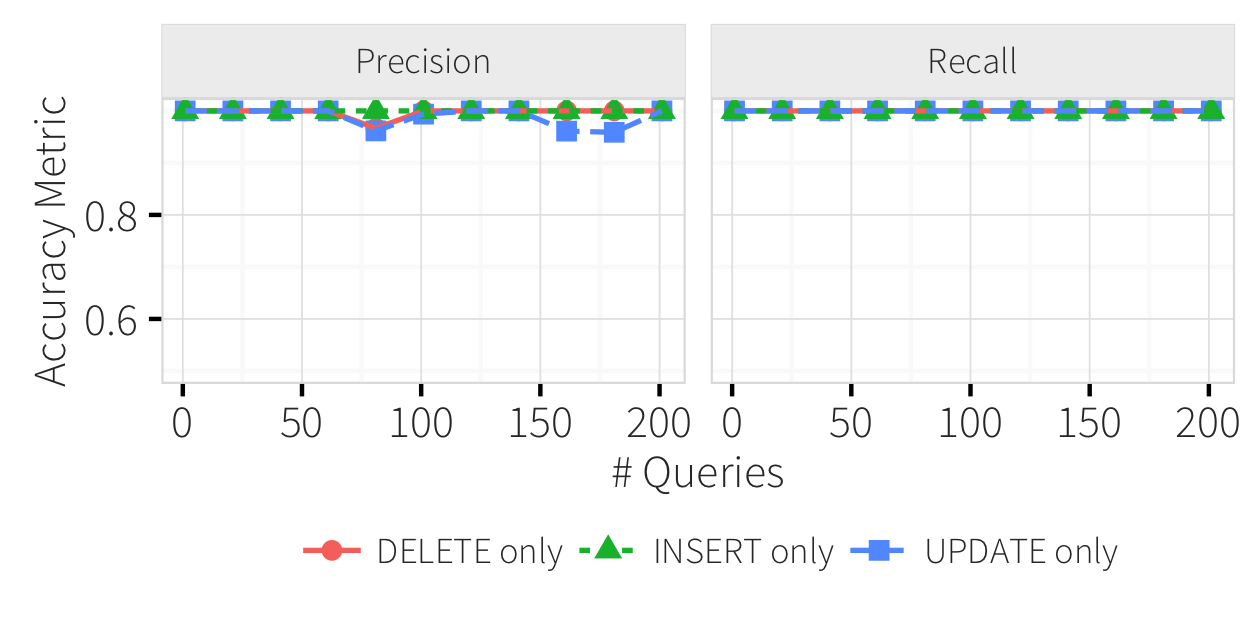
\includegraphics[width = .99\columnwidth]{figures/indelup_pr}
    \vspace*{-.25in}
    \caption{Accuracy for different query types.}
    \label{f:indelup_acc} 
    \end{subfigure}
    \vspace*{-.1in}
    \caption{Preliminary Experiments.}
  \end{figure*}
% \ewu{Should say this somewhere: 
% Updates are often a small fractice of a query workload -- typically $10\%$~\cite{} in most benchmarks --
% thus in practice \sys can work for much larger workloads.  In the experiments, we filtered the workloads to 
% only look at modification queries, and specifically UPDATE queries which are hard.
% }


In this section, we carefully study the performance and accuracy
characteristics of the basic MILP-based repair algorithm, as well as 
slicing-based optimizations that improve the latency of the system
, and an incremental algorithm for single query corruptions that
further improves the latency. 
%and 
%the multi-pass tuple-slicing algorithm that tolerates incomplete complaint sets with minimal loss in accuracy.
Our goals in the evaluation is to understand these trade-offs in
controlled synthetic scenarios, as well as study the effectiveness
in typical database query workloads based on widely used benchmarks.
\xlw{
By default, we set \sys as the incremental approach with tuple slicing optimization ($inc_1-tuple$) as it fixes our default synthetic query logs and benchmark workloads with minimum time cost and near perfect accuracy.
}


To this end, our experiments are organized as follows: First, 
we compare the basic and incremental MILP algorithm against the different optimizations 
to highlight the value of different optimizations.  We then compare the
repair costs of \texttt{INSERT}, \texttt{DELETE}, or \texttt{UPDATE}-only query logs 
and find that the latter query type is by far the most complicated and costly to repair.
For the subsequent experiments, we focus solely on \texttt{UPDATE}-only synthetic workloads 
to understand how \sys responds to different query logs and databases.  
We further evaluate the efficacy on real-world databases transaction benchmarks,
TPC-C and TATP. Finally, we evaluate \sys on a series of query logs with different properties. 
All experiments were run on 12x2.66 GHz  machines with 16GB RAM running CentOS release 6.6.



% establish the quality limitations of existing heuristics and the need for a formal, 
% constraint-based algorithm (\exact).  Second, we study how each of the 
% optimizations described in Section~\ref{s:optimiztaions} improves algorithm scalability.
% Third, we introduce different forms of error in the input complaint sets and study the 
% effectiveness of our noise-handling heuristics.  




%
% NOTE: figures are named <experimentsection>_<subsection>_<xaxis>.pdf
%

\subsection{Experimental Setup}


\iffalse
\begin{table}[t]\small
  \centering
  \begin{tabular}{@{}cll@{}}
  \toprule
  {\bf Param} & {\bf Description} & {\bf Default} \\ \midrule
  $V_d$  & Domain range of the attributes  & $[0, 100]$ \\
  $N_D$  & \# tuples in final database & $1000$ \\
  $N_a$  & \# attributes in database & $10$ \\
  $N_w$  & \# predicates in \texttt{WHERE} clauses & $1$ \\
  $N_s$  & \# \texttt{SET} clauses & $1$ \\
  $N_q$  & \# queries in query log & $300$ \\
  $idx$  & Index of corrupted query & $\{0, 25, 50,$ \\
         & (backwards from most recent) & $100, 200, 250 \}$ \\ %$\frac{N_q}{2}$ \\
  $r$    & Range size of \texttt{UPDATE} queries & 8 (tuples) \\
  $s$    & Zipf $\alpha$ param of query attributes, & $1$ \\ \bottomrule \end{tabular}
  %$set$  & Constant vs relative \texttt{SET} clauses. & const \\ 
         %& power low distribution $P(v) = v^{-s}$ & \\\end{tabular}
  \caption{Experimental Parameters}
  \label{t:params}
\end{table}
\fi


\iffalse
  \begin{table}[t]\small
    \centering
    \begin{tabular}{@{}cl@{}}
    \toprule
    {\bf Param} & {\bf Description} \\ \midrule
    $p$ & Precision: \% of repaired tuples that are correct. \\
    $r$ & Recall: \% of full complaint set repaired.\\
    % $t_{prep}$ & Time to construct CPLEX problem \\
    % $t_{send}$ & Time to send CPLEX problem to solver \\
    % $t_{solve}$ & Time for solver to generate a solutions\\
    $t_{total}$ & End-to-end execution time \\ 
    $d_{measure}$ & \red{Some sort of distance measure} \\ \bottomrule \end{tabular}
    \caption{Metrics Compared}
    \label{t:metrics}
  \end{table}
\fi




Each of our experiments follows a consistent procedure. 
We generate a sequence of queries using a synthetic query generator or 
the benchmark program, and corrupt the query log as described below. 
We then execute the original and corrupt query logs on an initial (possibly empty) database,
and perform a tuple-wise comparison between the resulting database states 
to generate a true complaint set.  
We then add noise to the complaint set by removing (partial) true complaints to simulate false negatives.
Finally, we execute the evaluated algorithms on the complaints and compare the fixed
query log with the true query log, as well as the fixed and true
final database states to measure performance and accuracy metrics.
\iffalse
We compare the following algorithms: 
\xlw{$\sys_{S \subseteq \{t,q,a,inc-x\}}$, where $S$ 
defines the set of optimizations present in the algorithm: 
the subscripts $t,q,a$ represent the
application of tuple, query and attribute slicing optimizations and $inc-x$ represents 
the incremental query repairs with step size {\it x}.
For example, $\sys_{tq,inc-1}$ uses both tuple and query slicing along with incremental repair with step size 1.}
\xlw{I removed the stop early and search all description here. Could be added later, current updated experiment do not contain results for this. }\ewu{Clearly define to the reader what "QFix" is.  It's used all over the place and not clear what it means.}
\fi
Performance is measured as wall clock
time between submitting a query log and the system terminating after retrieving a valid repair.  
We also measure the repair's precision (percentage of repaired tuples that were correctly fixed), 
the recall (the percentage of the full complaint set that was repaired), 
and the F1 measure (the harmonic mean of precision and recall).
Our reported metrics are the average across 20 runs.
%Finally, Table~\ref{t:params} summarizes the key parameters that we vary throughout our experiments.  
We describe the experimental parameters in the context of the datasets and workloads below.
\subsubsection{Datasets and Workloads}


This subsection describes the query and data generation process in greater detail.

\stitle{Synthetic:} \label{sec:syntheticgen}
We generate an initial database of $N_D$ random tuples.  
The schema contains $N_a$ attributes $a_1\ldots a_{i}$, whose values are integers
picked from $[0, V_d]$ uniformly at random, along with a primary key $id$. 
We then generate a sequence of $N_q$ \texttt{UPDATE} queries~\footnote{\scriptsize We focus on
\texttt{UPDATE} only query logs because they are the {\it predominant} cost 
in a query log.  Experiment~\ref{sec:indelup} compares \texttt{INSERT}, \texttt{DELETE} and \texttt{UPDATE}
only workloads to illustrate the difference.} in the format (SET and WHERE clauses) described as below. The default
setting for these parameters are: $N_D = 1000, N_a = 10, V_d = 200, N_q = 300$.
% UPDATE SET X,.. WHERE Y ...
{\scriptsize
\begin{verbatim}
  SET Clause:
   Constant: SET (a_i = ?),..
   Relative: SET (a_i = a_i + ?)
  WHERE Clause:
   Point:    WHERE a_j = ? AND ...
   Range:    WHERE a_j in [?, ?+r] AND ... 
\end{verbatim}
}
where \verb|?| is a randomly generated value and \verb|r| is the size of the range predicate. \\
\noindent \texttt{UPDATE} queries are composed of a combination of a SET clause 
can assign an attribute a $Constant$ or $Relative$ values (as shown above),
and a WHERE clause can either be a $Point$ predicate on a key, or a $Range$ predicate on non-key attributes.  
Note that a range predicate where \texttt{r = 0} is distinct from a $Point$ predicate due to the non-key attribute.
By default, we generate queries with non-key range predicates and constant set clauses.

% $X \& Y$ represents the \texttt{UPDATE} query type. $X$ represents the set clause type which can be either constant update ($Constant$) or
% relative update ($Relative$). Similarly, $Y$ represents the where clause type that can be either point update ($Point$) or
% range update ($Range$). Note that the 
% we default focus on \texttt{UPDATE} queries with non-key predicates on range(s) and constant SET clauses.
% 
% The \texttt{SET} clause sets the attribute to a random constant value in $V_d$ and 
% the \texttt{WHERE} clauses form a conjunction.  
% The $set$ parameter controls whether the \texttt{UPDATE} queries set attributes to random constant values ({\it const}),  
% or relative values ({\it rel}) by incrementing by a random, possibly negative, value.  
In addition, the skew parameter $s$ determines the distribution attributes referenced in the \texttt{WHERE} and \texttt{SET} clauses.  
Each attribute in a query is picked from either a uniform distribution when $s=0$ or a zipfian distribution.
This allows our experiments to vary between a uniform distribution, where each attribute is
equally likely to be picked, and a skewed distribution where nearly all attributes are the same. \\
The \texttt{WHERE} clauses in \texttt{DELETE} queries are generated in an identical fashion, while
\texttt{INSERT} queries insert values picked uniformly at random from $V_d$.

\stitle{TPC-C:} We use the data and query workload over the {\it ORDER} table in TPC-C~\cite{tpcc}.  
We generated a database at scale 1 with one warehouse, and kept the queries that modify the
{\it ORDER} table. The initial table contains 6000 tuples and we ultimately generated a log with
2000 queries, where $1837$ are \texttt{INSERT}s and the rest are \texttt{UPDATE}s. 

\stitle{TATP:} TATP workload simulates the 
caller location system. We generate a database from {\it SUBSCRIBER} table
with 5000 tuples and $2000$ \texttt{UPDATE} queries.\\
Both TPC-C and TATP setups were generated using the OLTP-bench project~\cite{difallah2013oltp}. 
We corrupt up to 1500 queries ahead of the most recent query.  



\stitle{Corrupting Queries:} We corrupt query $q_i$ by replacing it with a randomly
generated query of the same type based on the procedures described above.
To standardize our procedures, we selected a fixed set of indexes $idx$
that are used in all experiments.  
%Appendix~\ref{app:qidx} presents
%experiments that justify the rationale behind our selection.






% \begin{figure}[h]
% \centering
%   \begin{subfigure}[t]{\columnwidth}
%   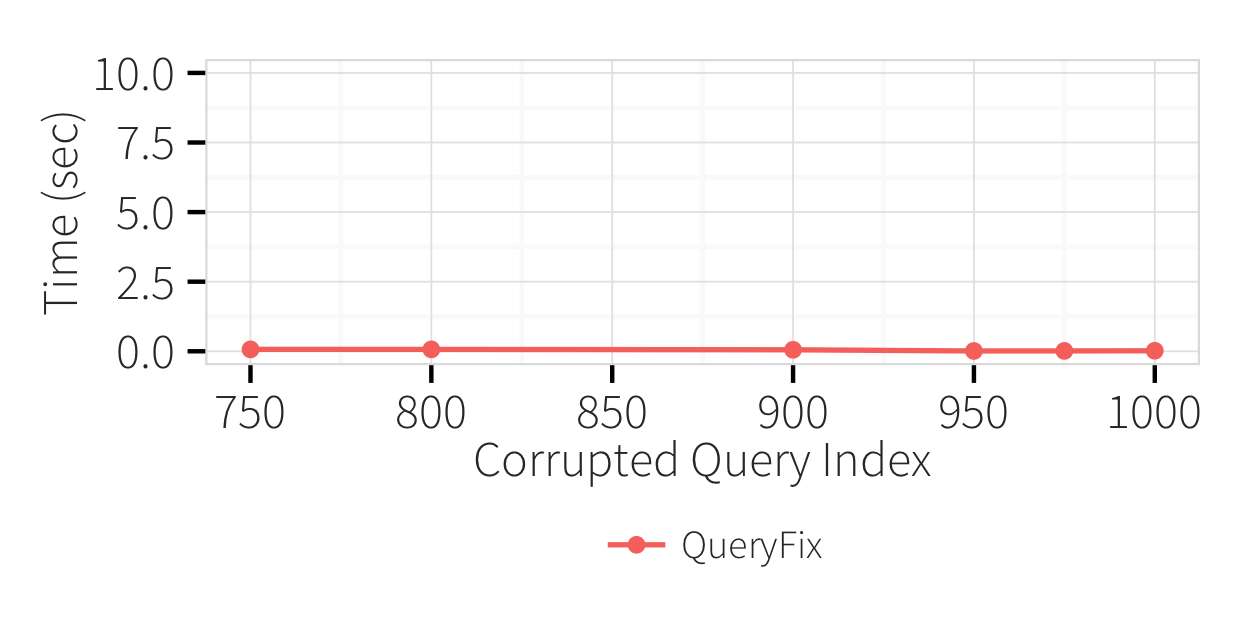
\includegraphics[width = .95\columnwidth]{figures/tpcc_time}
%   \caption{Performance on TPC-C Benchmark}
%   \label{f:tpcc} 
%   \end{subfigure}
%   \begin{subfigure}[t]{\columnwidth}
%   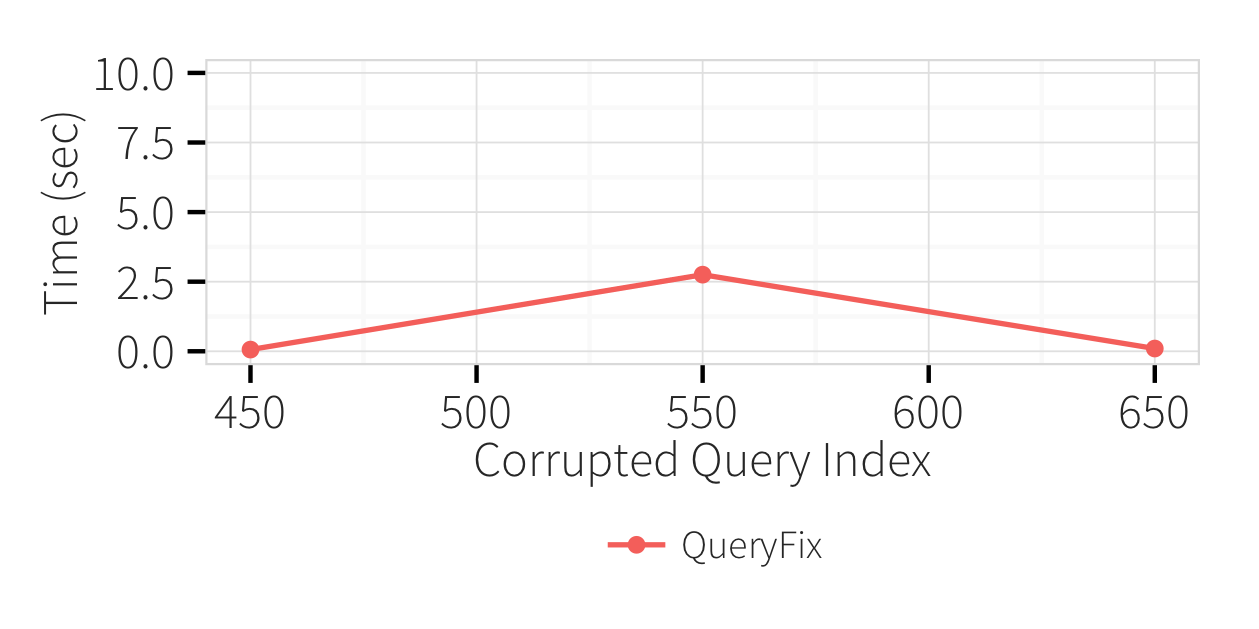
\includegraphics[width = .95\columnwidth]{figures/auction_time}
%   \caption{Performance on AuctionMark Benchmark}
%   \label{f:auctionmark} 
%   \end{subfigure}
%   \caption{Benchmark Performance}
% \end{figure}

\subsection{Preliminaries}
The following set of experiments are designed to establish the rationale for 
the settings in the subsequent experiments.  
Specifically, we compare different slicing-based optimizations of the basic approach
as the number of queries increases.  
We then evaluate the scalability of the different slicing-based optimizations of the 
incremental approach in the context of a single
corrupted query. We then establish the difficulty of repairing \texttt{UPDATE} 
workloads as compared to other query types. 

\stitle{Multiple Corrupt Queries:}
In this experiment, we compare the basic algorithm ($basic$) against 
each slicing optimization individually($basic-tuple, basic-attr, basic-query$) and all of them together ($basic-all$).  
We use the default settings with $N_D = 1000$ tuples and a sequence of \texttt{update} queries.
We generate query logs in 5 different sizes $N_q\in \{10, 20, 30, 40, 50\}$ and corrupt 
every tenth query starting from oldest query $q_1$,
up to $q_{41}$.  For example, when the $N_q = {30}$, we corrupt 3 queries: $q_{1,11,21}$. 
We find that the number of queries greatly affects both the scalabality (Figure~\ref{f:multi_time}) 
and the accuracy (Figure~\ref{f:multi_acc}) of the algorithms. Specifically, as the number increases,
the number of possible assignments of the MILP parameters increases exponentially and the solver often takes
longer than our experimental time limit of $1000$ seconds and returns an infeasibility error.  
This is a predominant reason why the accuracy degrades past $30$ queries.  For example, 
when $40$ queries are involved (with $4$ corruptions) 
and we ignore the infeasible executions, the average execution time is $300$ seconds
and the precision and recall are greater than $0.94$.  Unfortunately, with $50$ queries ($5$ corruptions),
all runs exceed the time limit and return infeasibility.

\stitle{Single Query Optimization:}
In this experiment, we evaluate the efficacy \sys with tuple slicing and incremental optimization
in the special case when only one query has been corrupted. \xlw{We compare 
\incremental without tuple slicing ($inc_1$) against tuple slicing at 
different batching levels of 1, 2, 8 ($inc_1-tuple; inc_2-tuple, inc_8-tuple$). Recall from Section~\ref{sec:incremental}, choosing $k$ batching level, we parameterize $k$ consecutive queries in batch from the most recent query until finding a valid fix.} \ewu{batching has not been introduced at all.  Need to describe in optimizations section and remind reader what it is here}. 
Figure~\ref{f:singlequeryinc_time} highlights the scalability limitation of the incremental 
algorithm without tuple slicing: with 50 queries $inc_1$ could easily runs exceed the 1000 seconds.   
In addition, Figure~\ref{f:singlequeryinc_acc} also shows a significant drop in accuracy as we increase the batching level from $1$ 
to $2$ as the failure rate of the MILP problem is positive proportional to the incremental batch level. 


\stitle{Query Type Experiment:}\label{sec:indelup}
Our final preliminary experiment evaluates the incremental algorithm with tuple slicing optimization 
($inc_1-tuple$) on \texttt{INSERT}, \texttt{DELETE}, or \texttt{UPDATE}-only workloads.
We increase the number of queries from $1$ to $200$ and corrupt the oldest query in the log.  
Figure~\ref{f:indelup_time} shows that while the cost of repairing \texttt{insert} workloads
remains relatively constant, the cost for \texttt{delete}-only and \texttt{update}-only workloads increase as 
the corruption happens earlier in the query log---and a much faster rate for \texttt{update} queries.
The F1 score for all settings is nearly 1 (Figure~\ref{f:indelup_acc}).


{\it Takeaways: we find that the basic \sys algorithms, even when using the slicing-based optimizations,
have severe scalability limitations due to the large number of undetermined values -- this is not surprising
since MILP constraint solving is a known NP-hard problem.
In contrast, we find that the incremental algorithms \ewu{with batch size of 1: emphasize it's single query incremental} are more effective at scaling to larger query log sizes.  
Furthermore, we show that \texttt{UPDATE}-only workloads are significantly more expensive to repair than other 
query types. Based on the result, we consider incremental
algorithm at batching level 1 with tuple slicing optimization ($inc_1-tuple$) as default setting in the rest of the experiment. In addition, we only consider \texttt{UPDATE}-only workload in synthetic experiments in Section~\ref{sec:experiments:synth}. 
}

 \begin{figure*}[h]
    \vspace*{-.1in}
    \centering
    \begin{subfigure}[t]{.45\textwidth}
    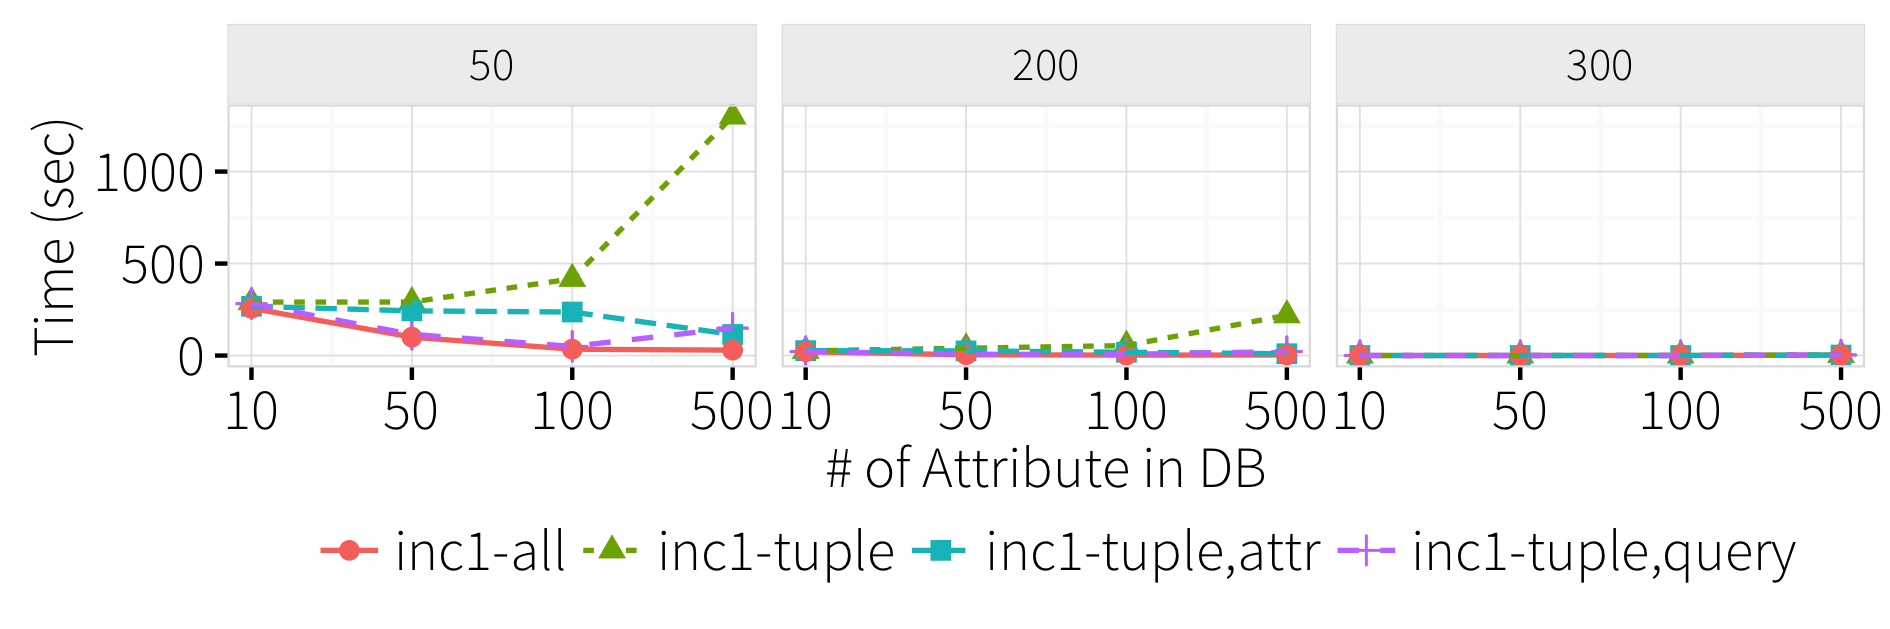
\includegraphics[width = .99\columnwidth]{figures/attr_time}
    \vspace*{-.1in}
    \caption{\# of Attribute vs. Time}
    \label{f:attr} 
    \end{subfigure}
    \begin{subfigure}[t]{.45\textwidth}
    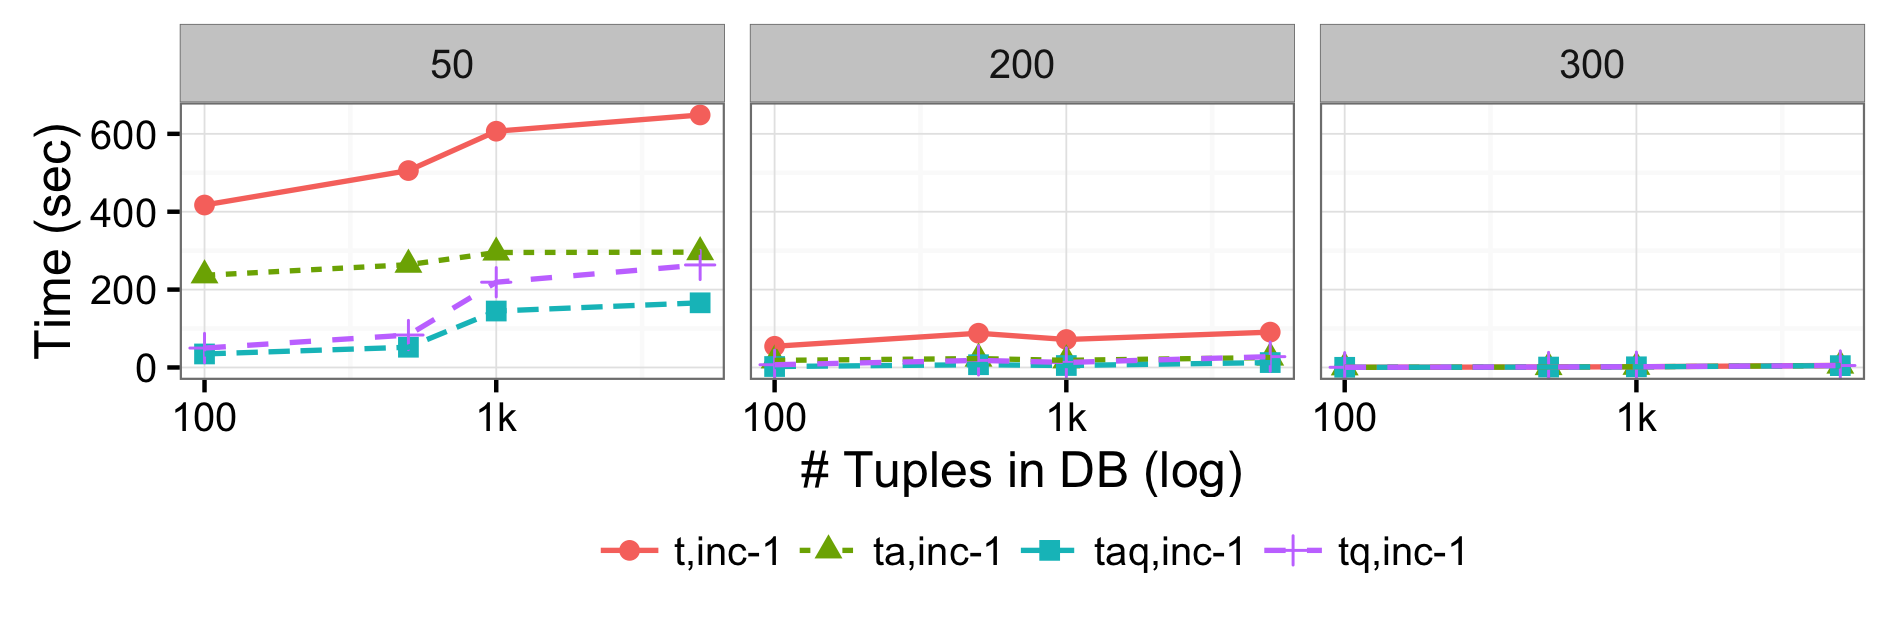
\includegraphics[width = .99\columnwidth]{figures/attr100_time}
    \vspace*{-.1in}
    \caption{Database Size vs. Time ($N_a = 100$)}
    \label{f:attr100} 
    \end{subfigure}
    \vspace*{-.1in}
    \caption{Comparison of Optimizations.}
  \end{figure*}
  
\subsection{Benchmarks \ewu{Move to last exp}}
\label{sec:experiments:benchmark}

Figure~\ref{f:tpcctatp} plots the performance of the \sys (incremental, tuple slicing)
on TPC-C and TATP benchmark applications.  In both workloads, \sys derives repairs efficiently.
And for TPC-C, \sys solves the problem on the order of milliseconds where all corrupted queries are \texttt{INSERT}s. 
The precision and recall measures were
$1$ both all settings.   One reason for the good performance is due to the fact that the benchmark queries
are pre-dominantly point \texttt{INSERT} or \texttt{UPDATE} queries.  In this setting, each tuples affects a very small set of 
tuples, which results in $1$ or $2$ complaints on average.  In this case, the tuple and query slicing algorithms
reduce the total number of constraints for almost every setting to less than $100$.


{\it Takeaway: many workloads in practice are dominated by point \texttt{UPDATE} queries.  In these settings,
 \sys is very effective at reducing the number of constraints and can derive repairs in nearly
 interactive latencies.}
\begin{figure}[h]
\centering
  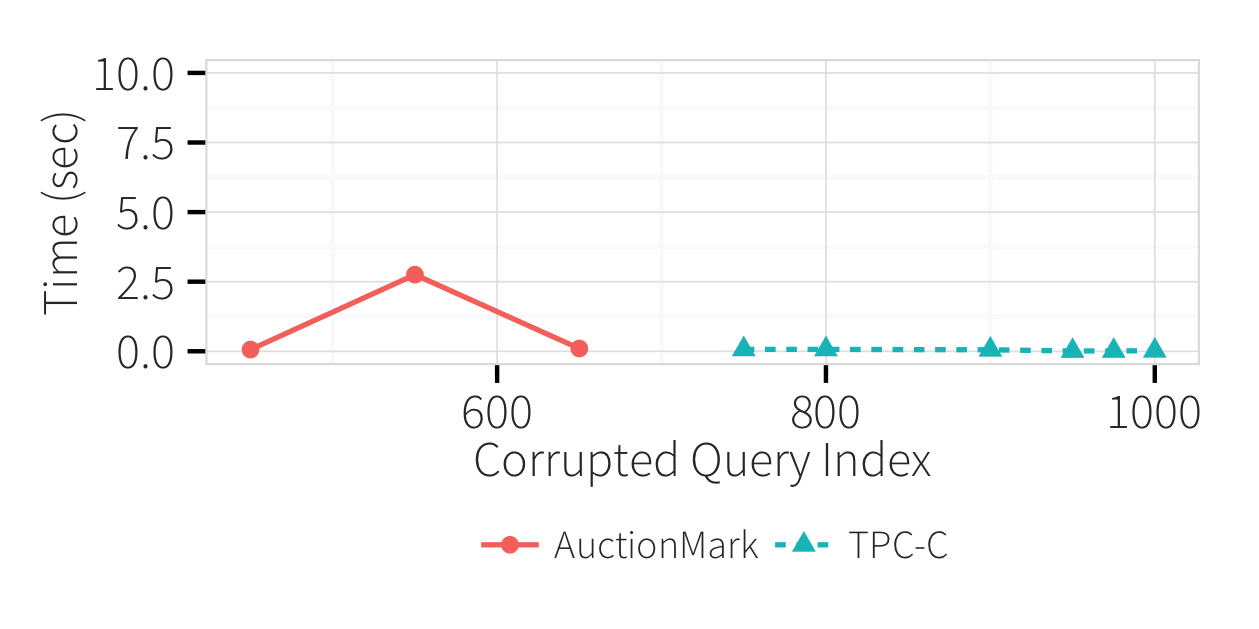
\includegraphics[width = .75\columnwidth]{figures/benchmark_time}
  \vspace*{-.2in}
  \caption{Performance on Benchmarks}
  \label{f:tpcctatp} 
  \vspace*{-.1in}
\end{figure}
\iffalse  
  \begin{figure*}[h]
    \centering
    \begin{subfigure}[t]{.3\textwidth}
      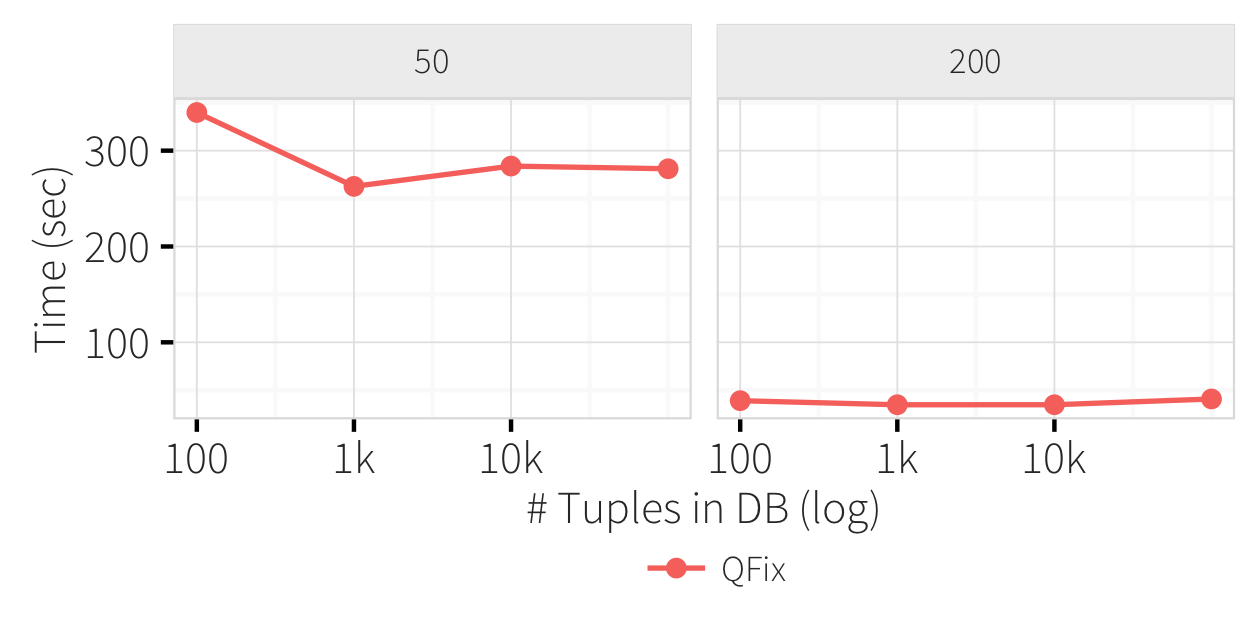
\includegraphics[width = .99\columnwidth]{figures/dbsize_time}
      \vspace*{-.1in}
      \caption{Database Size.}
      \label{f:dbsize_time} 
    \end{subfigure}
        \begin{subfigure}[t]{.3\textwidth}
      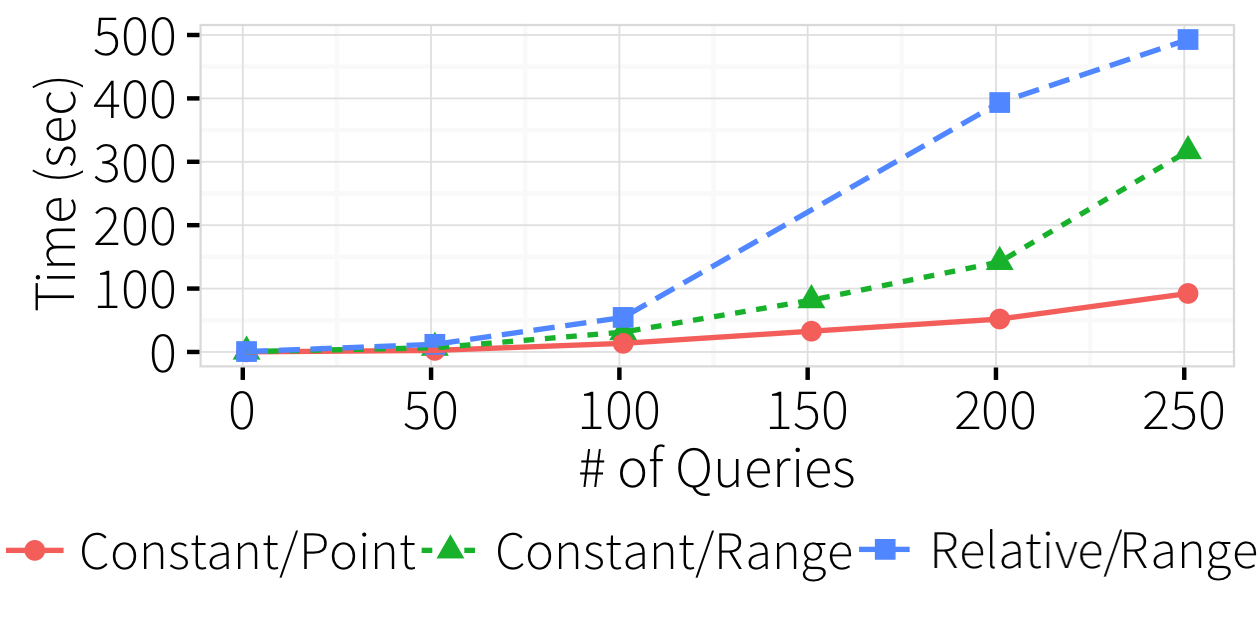
\includegraphics[width = .99\columnwidth]{figures/pointrelv_time}
      \vspace*{-.1in}
      \caption{Query Complexity (Query Type).}
      \label{f:qidx_time} 
    \end{subfigure}
    \begin{subfigure}[t]{.3\textwidth}
      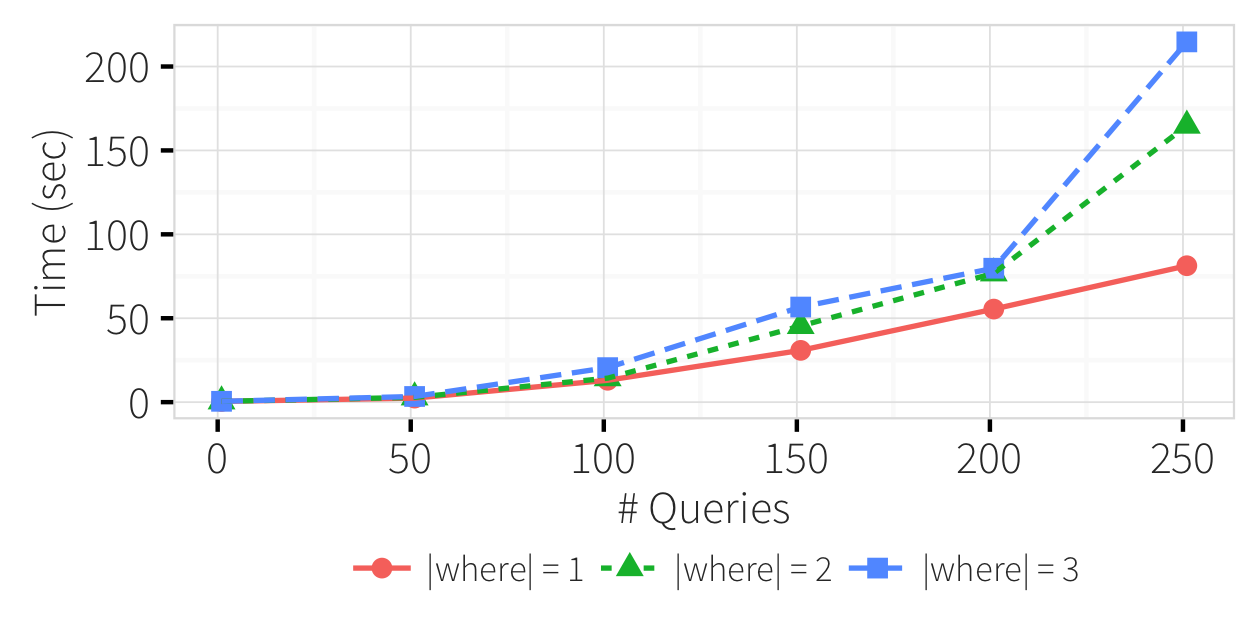
\includegraphics[width = .99\columnwidth]{figures/where_time}
      \vspace*{-.1in}
      \caption{Query Complexity (Where Size).}
      \label{f:where_time} 
    \end{subfigure}
    \\
    \begin{subfigure}[t]{.3\textwidth}
      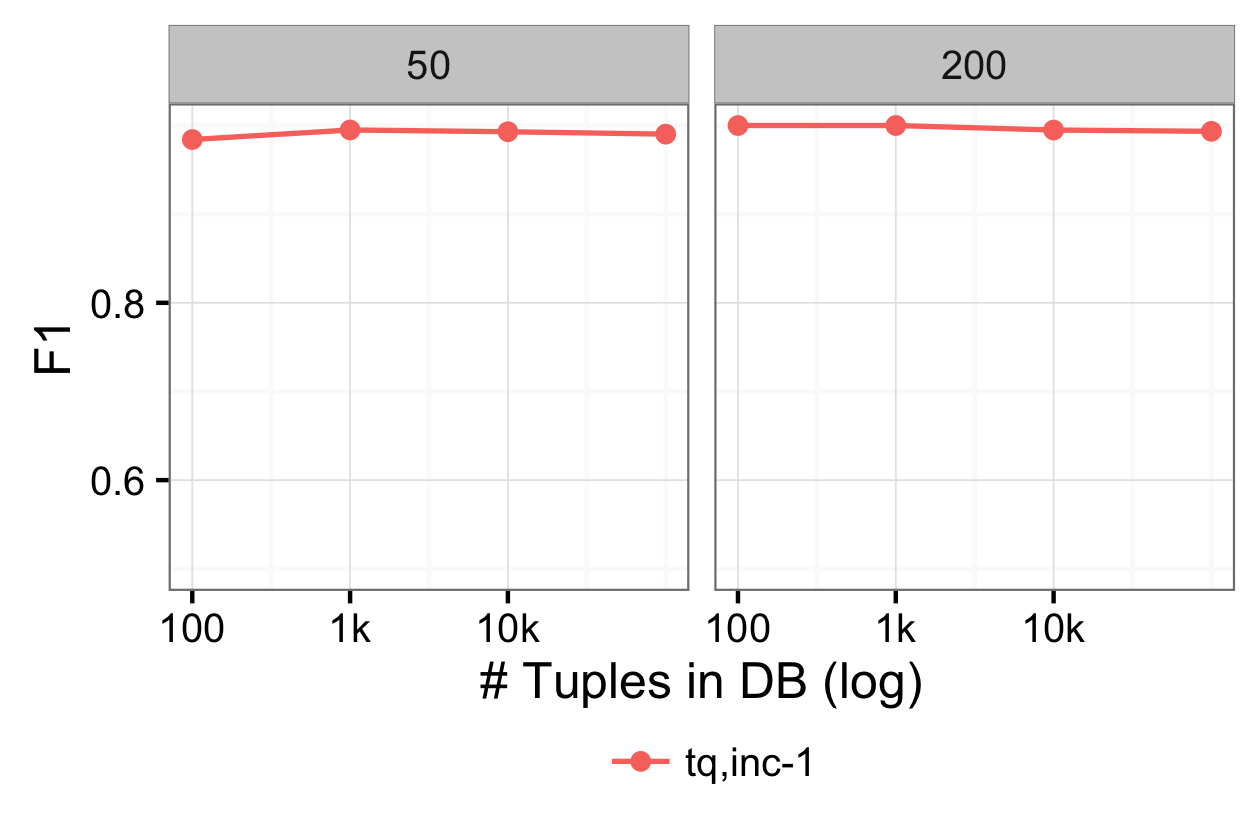
\includegraphics[width = .99\columnwidth]{figures/dbsize_acc}
      \vspace*{-.1in}
      \caption{Database Size vs F1-score. }
      \label{f:dbsize_acc} 
    \end{subfigure}
        \begin{subfigure}[t]{.3\textwidth}
      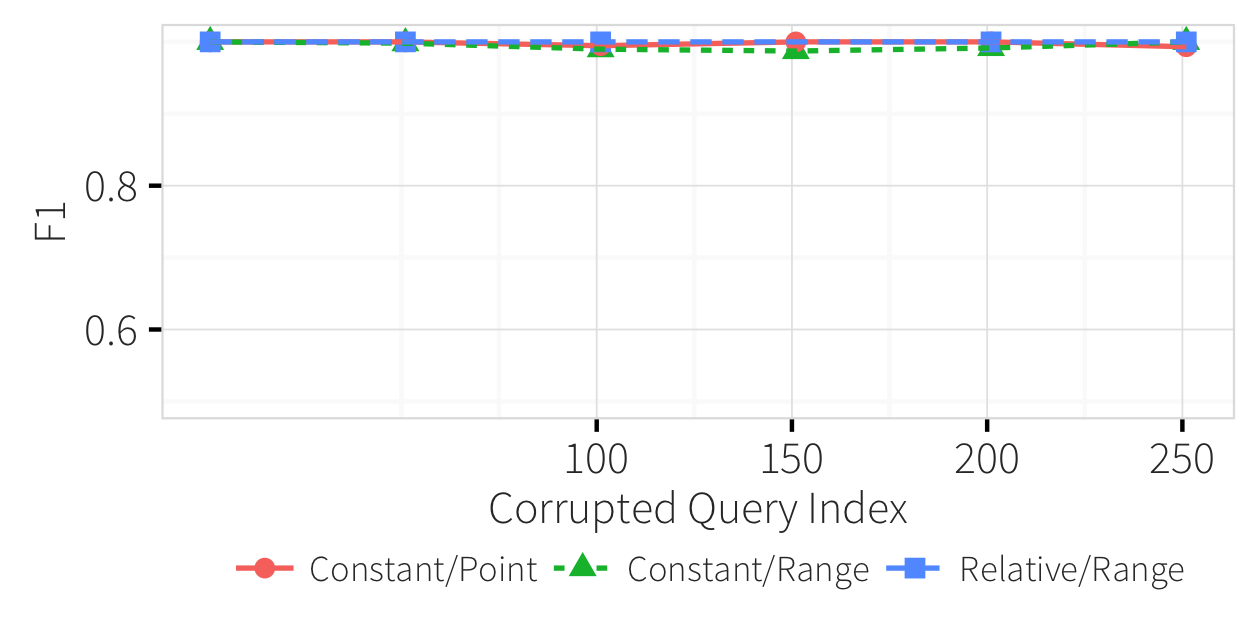
\includegraphics[width = .99\columnwidth]{figures/pointrelv_acc}
      \vspace*{-.1in}
      \caption{Query Complexity (Query Type) vs F1-score.}
      \label{f:qidx_acc} 
    \end{subfigure}
    \begin{subfigure}[t]{.3\textwidth}
      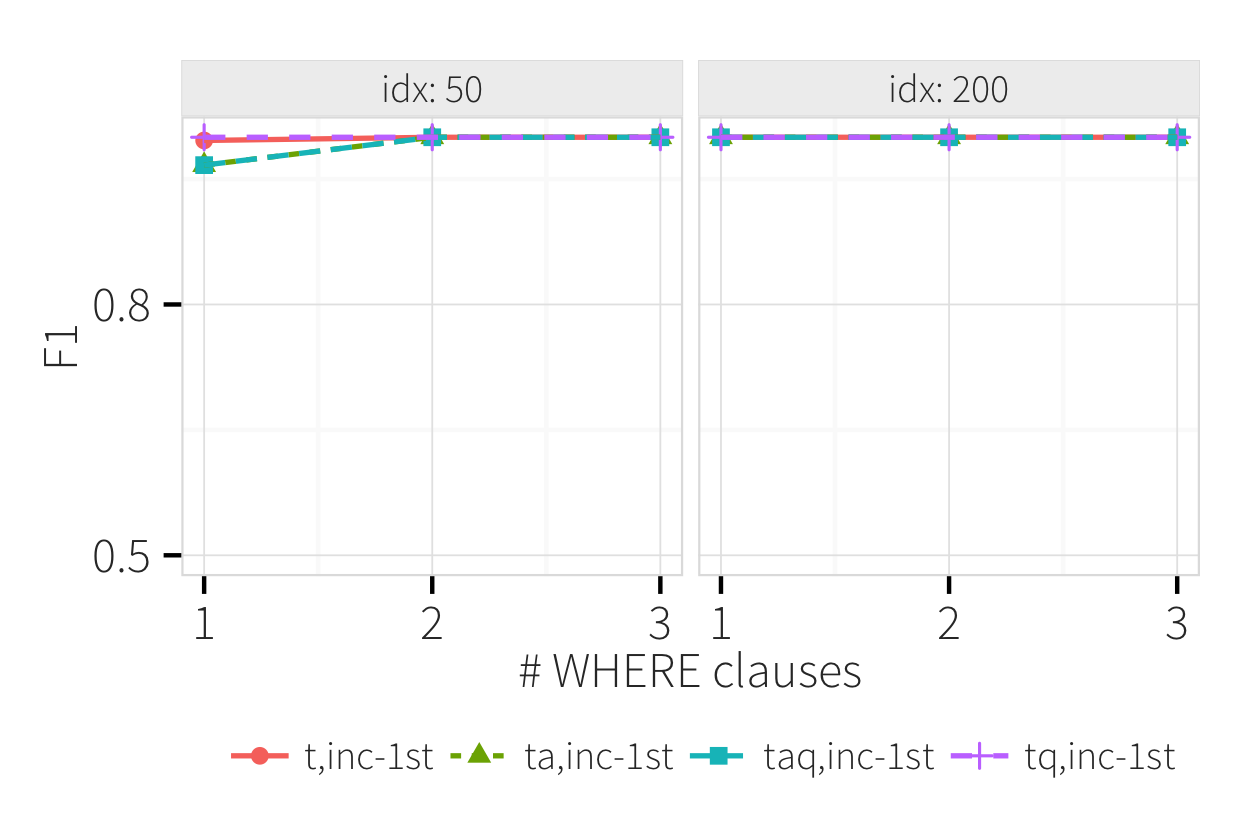
\includegraphics[width = .99\columnwidth]{figures/where_acc}
      \vspace*{-.1in}
      \caption{Query Complexity (Where Size) vs F1-score.}
      \label{f:where_acc} 
    \end{subfigure}
    
    \caption{Scalability Experiments (Performance)}
  \end{figure*}
\fi

\subsection{Synthetic Incremental Experiments}
\label{sec:experiments:synth}
We now perform a detailed evaluation of the incremental algorithm (batching level 1).
We divide these experiments into two groups: the first evaluates the difference slicing-based 
optimizations under different settings; the latter fixes the set of optimizations and varies workload and dataset parameters.
Note that we don't show accuracy figures for experiments with a $\ge 0.99$ F1-score.

\subsubsection{Comparing Optimizations}

\stitle{Varying \# Attributes}
We first evaluate \sys and its optimizations by increasing the number of attribute ($N_a$)
in the table from $10$ to $50, 100, 500$ with $N_D = 100$. As shown 
in Figure~\ref{f:attr}, when the number of attribute in a table is small, e.g., 10, 
performance of \sys with or without query slicing or attribute slicing optimizations 
appears identical. However, as we gradually increase the number of attribute, the benefit
of query slicing or attribute slicing become much more significant. 
In particular, applying all slicing optimizations ($inc_1-all$) is $40\times$ faster than \sys with only tuple-slicing 
optimization ($inc_1-tuple$) when there are 500 attribute in the table.  

\stitle{Database Size:}
We further increasing the database size $N_D \in \{100,500, 1k, 5k\}$ while keeping the number of attributes fixed at $N_a = 100$. 
\xlw{
As shown in Figure~\ref{f:attr100}, approach with all optimizations ($inc_1-all$)
shows constant percentage of efficiency gain over with only tuple-slicing optimization as the database size increases.} \ewu{What does this sentence mean?  gain over what?}.

\subsubsection{Sensitivity to Data and Workload Factors}

In the following set of synthetic experiments, we \ewu{focus on a single \sys setting---incremental with tuple-slicing---} and
individually vary numerous database and workload parameters in order to tease apart the algorithm performance.  
These include factors such as query complexity, log size $N_q$, database size $N_D$) and the skew of the query predicates.
We focus on a narrow table setting that contains $N_a = 10$ attributes, and a single corrupt query in the query log.
% Motivated by our preliminary results, we focus on \texttt{UPDATE}-only query logs with a single corruption with
% $10$ attributes and $1k$ attributes in the table. As the performance of \sys with different optimizations appears 
% identical when $N_a = 10$, we will only show results of \sys with tuple slicing optimization in the rest of the 
% experiments. 
  \begin{figure*}[h]
    \vspace*{-.1in}
    \centering
     \begin{subfigure}[t]{.3\textwidth}
      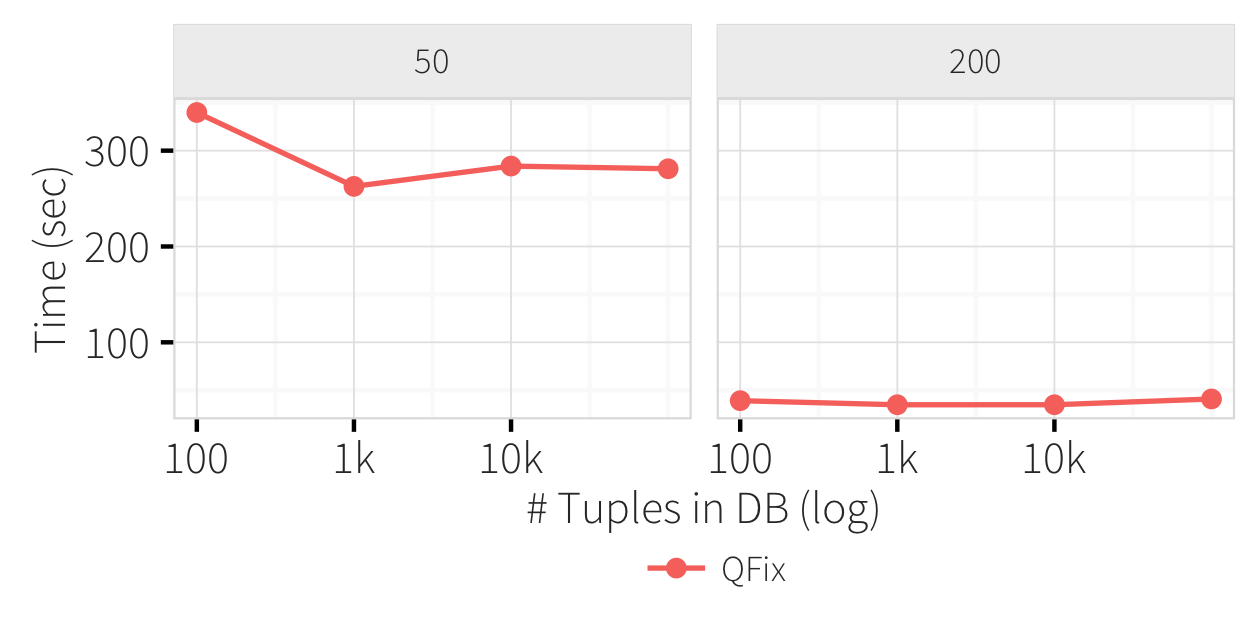
\includegraphics[width = .99\columnwidth]{figures/dbsize_time}
      \vspace*{-.2in}
      \caption{Database Size.}
      \label{f:dbsize_time} 
    \end{subfigure}
        \begin{subfigure}[t]{.3\textwidth}
      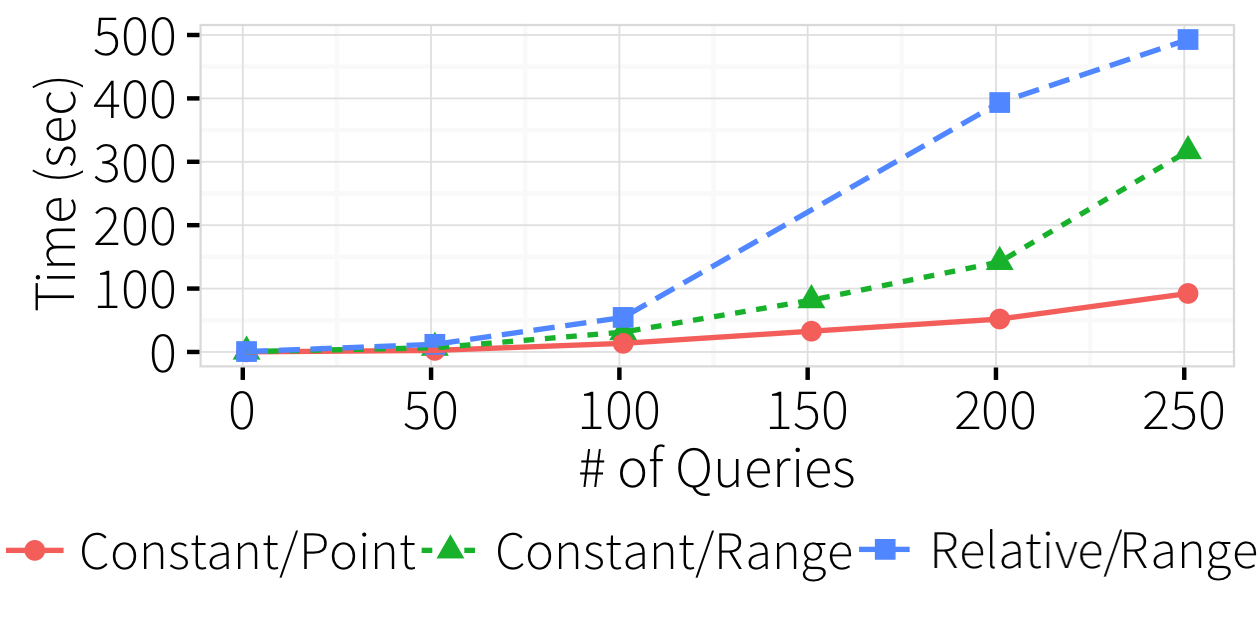
\includegraphics[width = .99\columnwidth]{figures/pointrelv_time}
      \vspace*{-.2in}
      \caption{Query Complexity (Query Type).}
      \label{f:qidx_time} 
    \end{subfigure}
    \begin{subfigure}[t]{.3\textwidth}
    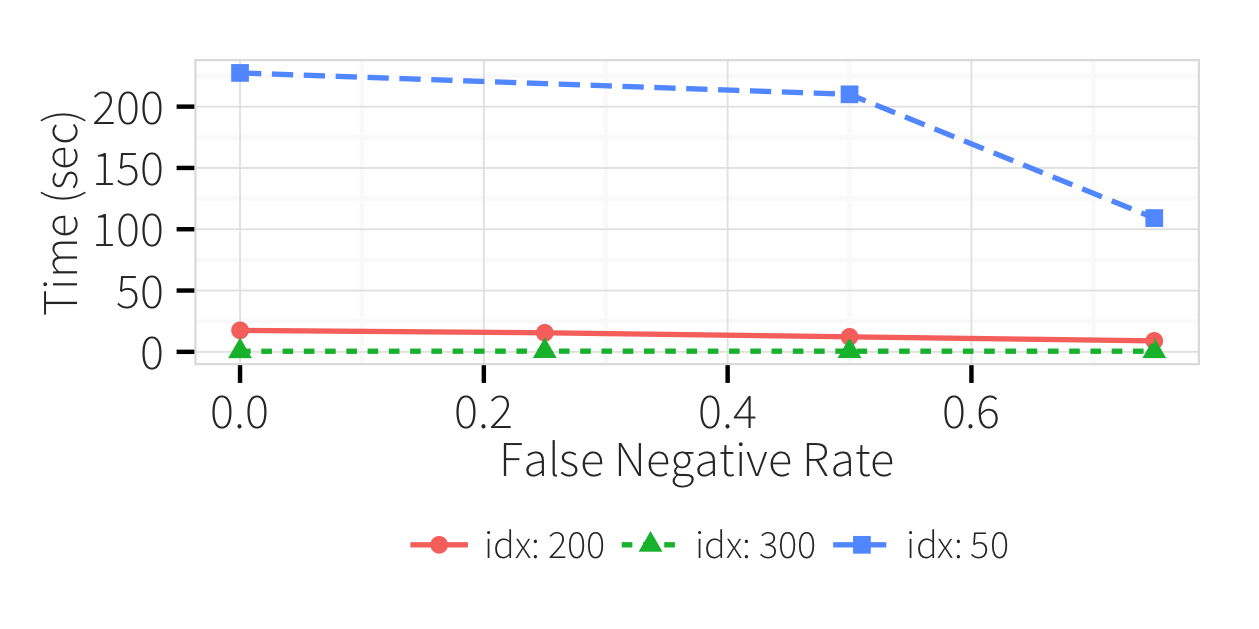
\includegraphics[width = .99\columnwidth]{figures/noise_fn_time}
    \vspace*{-.2in}
    \caption{Time vs False Negative}
    \label{f:falsenegative_time} 
    \end{subfigure} 
    \\
    \begin{subfigure}[t]{.3\textwidth}
    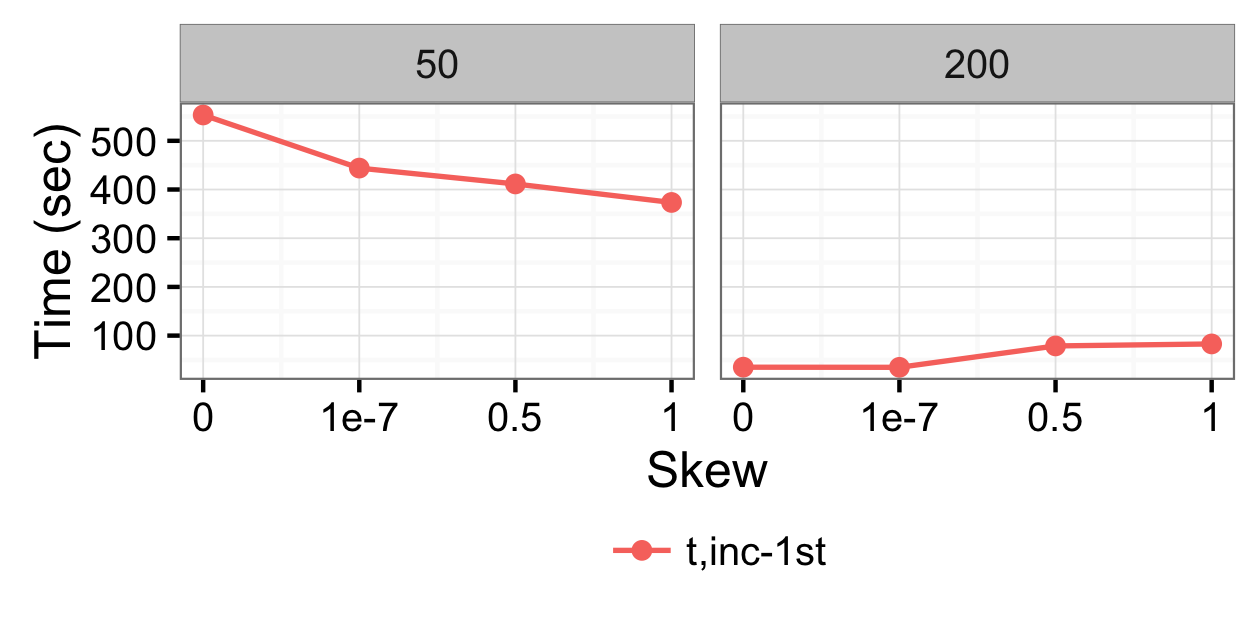
\includegraphics[width = .99\columnwidth]{figures/skew_time}
    \vspace*{-.2in}
    \caption{Skew vs Time}
    \label{f:skew_time} 
    \end{subfigure}
	\begin{subfigure}[t]{.3\textwidth}
      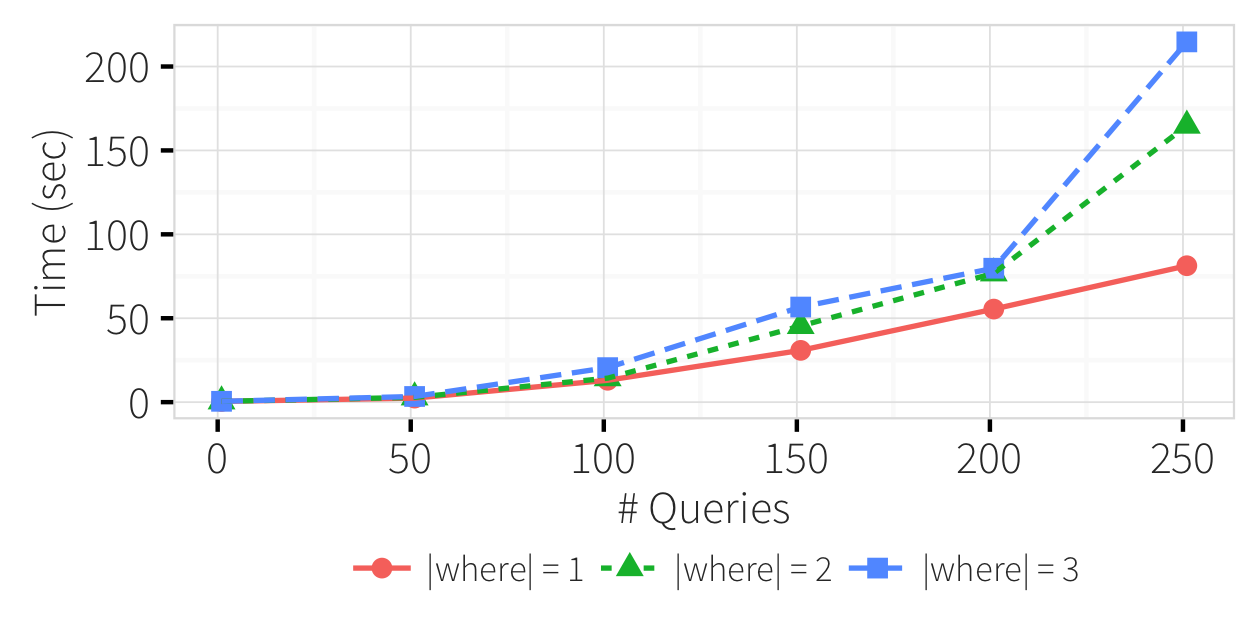
\includegraphics[width = .99\columnwidth]{figures/where_time}
      \vspace*{-.2in}
      \caption{Query Complexity (Where Size).}
      \label{f:where_time} 
    \end{subfigure}
    \begin{subfigure}[t]{.3\textwidth}
    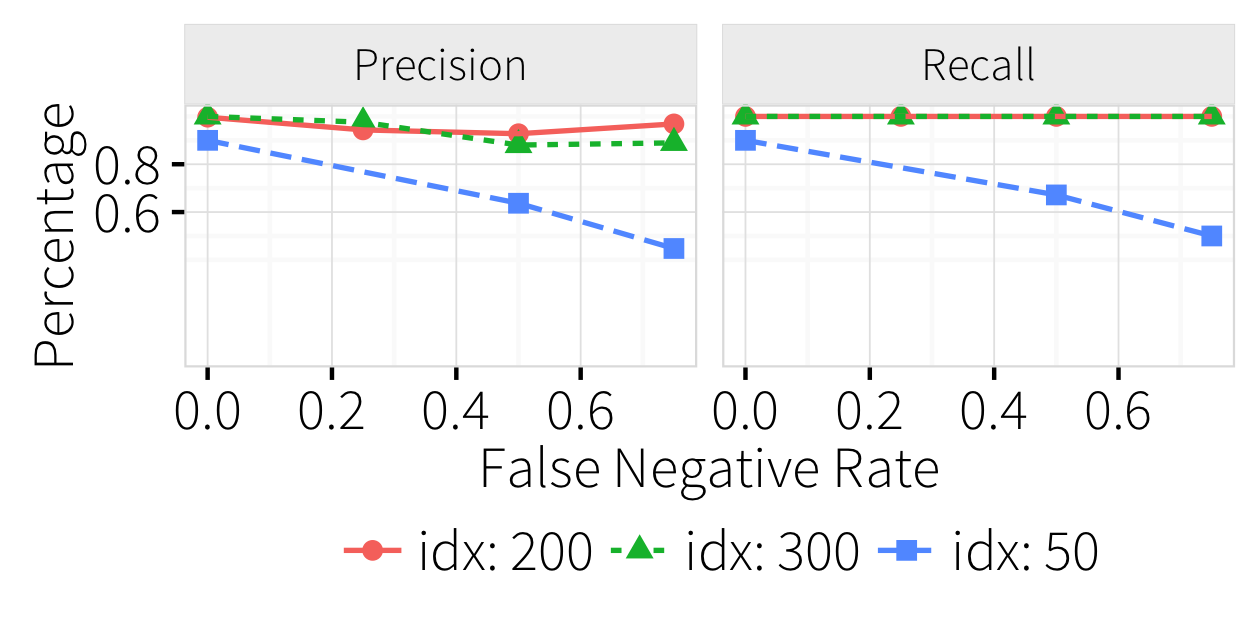
\includegraphics[width = .99\columnwidth]{figures/noise_fn_acc}
    \vspace*{-.2in}
    \caption{F1-score vs False Negative}
    \label{f:falsenegative_acc} 
    \end{subfigure}
    \vspace*{-.1in}
    \caption{Skew and False Negative experiments. }
  \end{figure*}
  \vspace*{-0.1in}


\iffalse 
\stitle{Scalability - Log Size:}
Figures~\ref{f:logsize_time} and~\ref{f:logsize_acc} increase the query log size (each subplot) between $50, 100, 500$ and $1000$.
We compared the baseline $\sys_{t,inc}^{1st}$ with addition attribute, query or both slicing optimizations.
For readibility purposes, we have normalized the x-axis to show the distance of the corrupted query from the most recent query in the log
(e.g., $x=50$ denotes that $q_{N-50}$ was corrupted).
As expectied, the cost increases as the corruption is older in the query log since more queries need to be tested before the
true corruption is encountered.  There algorithms all execute at roughly the same performance, though there is a slight advantage to
using the query-slicing optimization. The optimization reduces the time to linearize the query log by roughly $20\%$, however
the CPLEX solver time contributes to over half the total time so the improvement is difficult to see.
All algorithms exhibit near perfect F1-scores.
\fi


\stitle{Database Size:}
Figure~\ref{f:dbsize_time} varies the database size from $100$ to $100$k tuples \xlw{while setting the $V_d$ proportionally and other parameters to default in order to maintain the same query selectivity across different database sizes}.
For simplicity, we plot the performance and accuracy of corruptions at two query indexes: $50$ and $200$.
The more recent corruption ($200$) is executed in nearly constant time as the database size increases, with a perfect F1-score. \xlw{Meanwhile, as we increase the database size, \sys achieves near constant time cost after database size greater than 1k. The reason is as we maintain the same query selectivity, the number of complaints maintains roughly the same when database size increases. And the performance of the solver in dependent on the number of complaints. However, small database size may increase the randomness in query selectivity, thus we observe different time cost when database size is 100. 
}

\stitle {Query Type: }
So far, we have focused on \texttt{UPDATE} queries with constant set clauses and range predicates.  Figure~\ref{f:qidx_time} compares the other types of \texttt{UPDATE} queries: 
{\it Constant/Point, Constant/Range}, and {\it Relative/Range}. We also vary the size of the query log, while corrupting $q_1$.
%while increase the number of queries \sys need to solve from $1$ to $250$ (by adjusting the corrupt query index). 
\xlw{
As expected, point predicates are easier to solve than range predicates and constant set clauses are easier to solve than relative set clauses. The reason for the first observation is obvious since the cost for searching all valid values is far cheaper than searching all valid ranges. For the latter observation, we believe there are two reasons:
1. constant set clauses disconnect tuple values from query to query whereas relative set clauses maintain this connection. Thus, the searching space for the relative set clauses is often bigger than the constant one; 
2. since relative set clauses maintain the tuple value connection, their complaint set sizes are normally larger than constant set clauses for the same corrupt index: In relative set clauses, incorrectness always inherits from previous database state and could infects other tuples, however, this is less likely to happen for constant set clauses.}

\stitle{Query Predicate Dimensionality:}
Figure~\ref{f:where_time} varies the dimensionality of the update queries by increasing the number of predicates in the \texttt{WHERE} clause, while keeping the overall selectivity constant.
From Figure~\ref{f:where_time}, we found that more predicates increases the cost in solving a problem. 
This is expected as when there are more predicates, the number of constraints and variables in the MILP problem also increase, which further increase the problem complexity.
%We find that the performance improves as the number of predicates increases.
%This counter-intuitive result is due to the reduction in the complaint set size as the complexity increases. 
%Again, we omit the accuracy result as \sys exhibit above 0.996 average F1 score in all settings. 


\stitle{Skew:} We now study the effects of attribute skew on the algorithms.
We vary the skew parameter from $0$ (uniform) to $1e-7, 0.5$, and $1$. When $s=1$, nearly every attribute is $A_0$.
\xlw{
Higher skewness factor increases the update frequency of certain attributes, which further increases the number of constraints on these attributes. With more constraints, the searching space get reduced and thus the problem becomes easier to solve. The update frequency of an attribute is a combined result of the skewness factor and the number of queries in the problem: one would only observe the (frequency) difference when there are enough number of queries. 
Thus
we observe a clear decreasing trend in Figure~\ref{f:skew_time} as we increase the skewness factor on corrupt index equals to $50$ ($250$ queries from the most recent one). 
However, when the corruption is more recent (corrupt index equals to $200$, $50$ queries to the most recent one), this trend \sout{can be hardly seen} is less significant.
}

% 
% Our hypothesis is that higher skew results in a larger number of relevant queries, thus limiting the effectiveness of query slicing.
% In addition, recall that each query sets all tuples within the same range to the same value.  
% Since increasing the skew makes it more likely that both the \texttt{SET} and \texttt{WHERE} clauses reference the same attributes,
% it causes the tuples to cluster around the values, thus increasing the selectivity of the queries.
% This results in a larger complaint set, which 
% 
% with high skew, each query is more likely to modify the same tuples, thus increasing the number of
% 
% We generate query log at 4 different skewness levels from uniform to 
% super skewed with $s = 0, 1e-7, 0.5, 1$. As we can see as query log
% is more skewed, the execution time for solving same amount of queries 
% increase. This is also due to the fact that increasing skewness also
% increase the query dependency, which, in turn, increase the searching
% space in the MILP problem.


\stitle{Incomplete Complaint Sets:}
Our final experiment (Figures~\ref{f:falsenegative_time} and~\ref{f:falsenegative_acc}) varies the fase positive rate in incomplete complaint sets.
We increase the rate from $0$ ($0\%$ missing in the complaint set) to $.75$ ($75\%$ are missing).  
We find that reducing the size of the submitted complaint set naturally improves the repair performance,
however the repair quality, both precision and recall in Figure~\ref{f:falsenegative_acc}, may suffer if the corruption occured in a very old query. \xlw{This is expected since \sys targets on fixing complaints that are reported, thus with 
incomplete complaint, \sys may failed to fix false negative complaints and this results in low recall. Meanwhile, with missing complaints, \sys may end up with repairs that resolve all the reported complaints but indeed overfix correct tuples and this results in low precision. } 
\ewu{Do we have a good reason why?}


%   \begin{figure}[h!]
%     \centering
%     \begin{subfigure}[t]{\columnwidth}
%     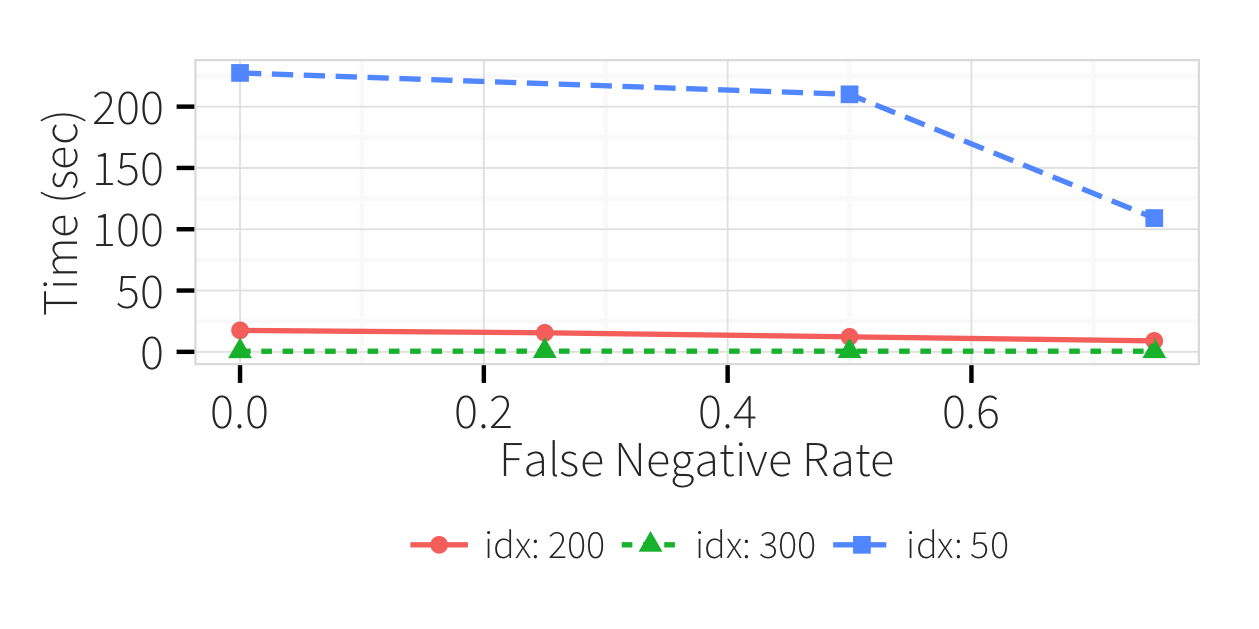
\includegraphics[width = .9\columnwidth]{figures/noise_fn_time}
%     \caption{Time vs Incomplete Complaint Size}
%     \label{f:falsenegative_time} 
%     \end{subfigure}
%     \begin{subfigure}[t]{\columnwidth}
%     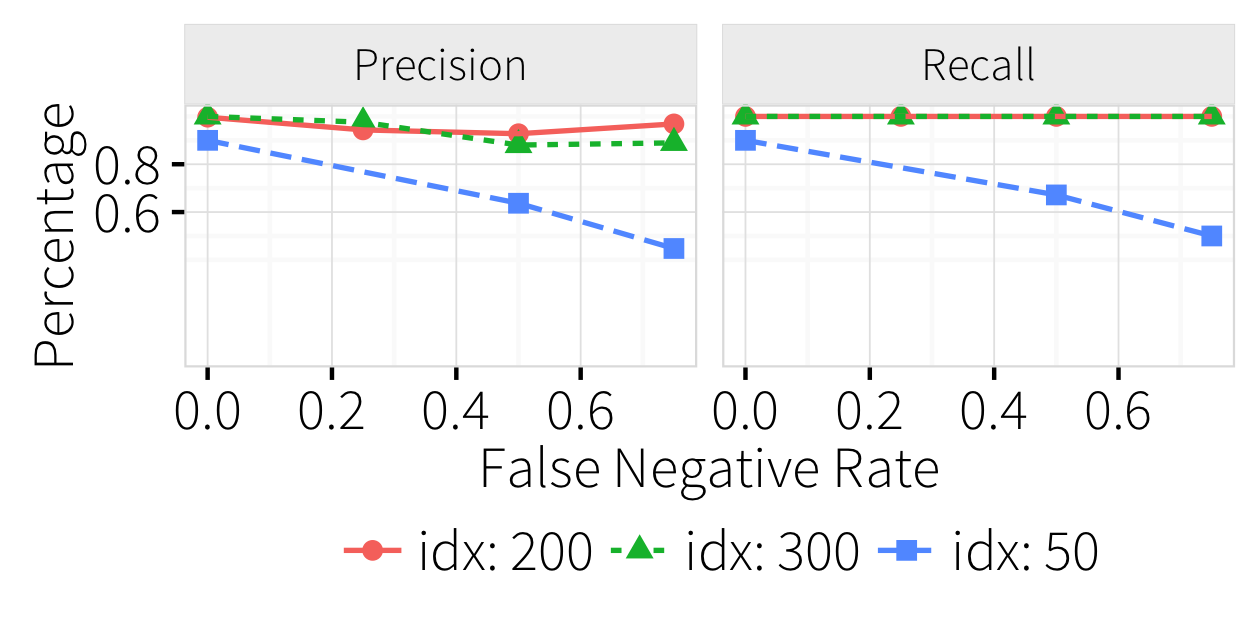
\includegraphics[width = .9\columnwidth]{figures/noise_fn_acc}
%     \caption{F1-score vs Incomplete Complaint Size}
%     \label{f:falsenegative_acc} 
%     \end{subfigure}
%     \label{f:falsenegative}
%     \caption{Incomplete Complaint Experiments}
%   \end{figure}
% 

\smallskip

\textit{Takeaways: we find that the performance of the different repair algorithm 
heavily depends on the property of the property of the datasets and the 
number of complaints in the complaint set. Attribute and query slicing show significant gain for 
datasets with large number of attributes. And the proposed \sys algorithm is able to solve hard problems
(with ~$200$ \texttt{UPDATE} queries) in reasonable amount of time. }
% \stitle{Incremental Results}
% INcremental algorithm, incremental results














